\begin{frame}\frametitle{Neutrino Oscillations Discovery}
\scriptsize
History of the neutrino oscillations discovery is described in the Griffiths textbook \cite{ref_Griffiths}, chapter 11.
\begin{itemize}
  \scriptsize
  \item Homestake experiment, 1968
  \begin{itemize}
     \scriptsize
     \item Chlorino radiochemical detector ($\nu_e + ^{37}Cl \rightarrow ^{37}Ar+e$) 
     \item Sensitive to $\nu_e$ only 
     \item Recorded $1/3$ of theoretically predicted neutrino flux
     \item Solar neutrino problem postulated
  \end{itemize}
  \scriptsize
  \item Bruno Pontecorvo proposed theory: neutrino can change flavor and, therefore, $\nu_e$ converted to $\nu_\mu$ and/or $\nu_\tau$ and weren't registered by Homestake experiment. But at first it was believed the experiment made mistake
  \item Over years, more neutrino experiments reported deficit of the Solar electron neutrinos
\end{itemize} 
\end{frame}

\begin{frame}\frametitle{Neutrino Oscillations Discovery}
\begin{itemize}
  \scriptsize
  \item Super-Kamiokande experiment, 1998 
  \begin{itemize}
     \scriptsize
     \item Water Cherenkov detector ($\nu + e \rightarrow \nu + e$). 
     \item Sensitive to all $\nu$ but detection efficency of $\nu_e$ is 6.5 times bigger ($\nu_e$ has extra Feynmann diagrams with W-boson)
     \item Recorded $45\%$ of theoretically predicted neutrino flux (assumed all $\nu$=$\nu_e$)
  \end{itemize}
  \scriptsize
  \item Solar neutrino observatory (SNO), 2002
  \tiny
  \begin{itemize}
     \scriptsize
     \item Heavy water Cherenkov detector ($\nu_e + d \rightarrow p+p+e$, $\nu+d \rightarrow n+p+\nu$, $\nu+e \rightarrow \nu+e$)
     \item Sensitive to all $\nu$ but can separate $\nu_e$
     \item Reported $\nu_e$ flux to be $35\%$ of the predicted flux
  \end{itemize}
  \scriptsize
  \item Combining Super-Kamiokande and SNO results
  \begin{itemize}
     \scriptsize
     \item $45\%=35\%+10\%$, $10\% \cdot 6.5 = 65\%$, $35\%+65\%=100\%$
     \item Neutrino oscillations theory confirmed
     \item Solar neutrino problem resolved
  \end{itemize}
\end{itemize} 
\begin{figure}
\label{fig:NuScattering}
\centering
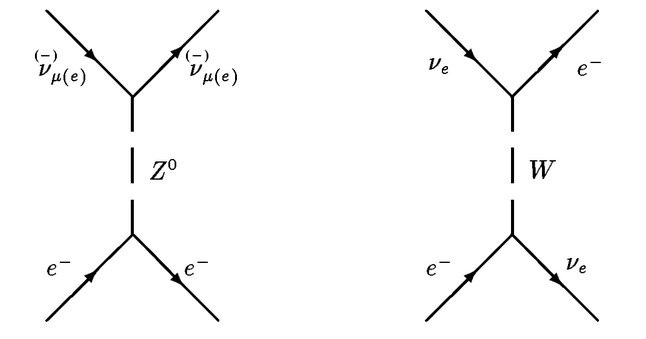
\includegraphics[width=0.60\textwidth, keepaspectratio=true]{figs/nuScattering_Only2.png}
\end{figure}
\end{frame}

\begin{frame}\frametitle{Theory. Two Neutrinos Case}
  \scriptsize
  \begin{center}
  $\nu_1=\nu_{\mu}cos\theta-\nu_esin\theta$\\
  $\nu_2=\nu_{\mu}sin\theta+\nu_ecos\theta$\\
  \end{center}
  \begin{center}
  $\nu_1(t)=\nu_1(0)e^{\frac{-iE_1t}{\hbar}}$, $\nu_2(t)=\nu_2(0)e^{\frac{-iE_2t}{\hbar}}$ $\leftarrow$ from quantum mechanics\\
  \end{center}
  Suppose, at t=0 there were $\nu_e(0)=1$, $\nu_\mu(0)=0$\\
  After calculations (\cite{ref_Griffiths}, chapter 11): 
  \begin{center}
  $P_{\nu_e \rightarrow \nu_\mu}=|\nu_\mu(t)|^2=[{sin2\theta}sin{\frac{(E_1-E_2)t}{2\hbar}}]^2=[{sin2\theta}sin{\frac{(m_1^2-m_2^2)c^3}{4\hbar{E}}z}]^2$\\  
  \end{center}
  \large $\rightarrow$\\
  \scriptsize
  For oscillations to happen, the following conditions must be satisfied:
  \begin{itemize}
     \item $\theta \neq 0$ (neutrino mixing presents)
     \item $m_1^2-m_2^2 \neq 0$ (neutrinos are massive and masses are different)
  \end{itemize}
\end{frame}

\begin{frame}\frametitle{Theory. Three Neutrinos Case}
  \scriptsize
  Mixing is determined by Pontecorvo-Maki-Nakagava-Sakata (PMNS) matrix:\\
  \begin{center}
  $ \begin{pmatrix} \nu_{e} \\ \nu_{\mu} \\ \nu_{\tau} \\ \end{pmatrix}
  = U_{PMNS}\cdot \begin{pmatrix} \nu_{1} \\ \nu_{2} \\ \nu_{3} \\ \end{pmatrix} = 
  \begin{pmatrix}
  U_{e1} & U_{e2} & U_{e3} \\
  U_{\mu1} & U_{\mu2} & U_{\mu3} \\
  U_{\tau1} & U_{\tau2} & U_{\tau3} \\
  \end{pmatrix}
  \cdot
  \begin{pmatrix} \nu_{1} \\ \nu_{2} \\ \nu_{3} \\ \end{pmatrix}$\\
  \end{center}
  $U_{PMNS}$ depends on neutrino mixing angles $\theta_{12}$, $\theta_{23}$, $\theta_{13}$ and CP-violating phase $\delta_{CP}$\\
  Define $c_{ab}=cos\theta_(ab)$, $s_{ab}=sin\theta_(ab)$\\
  \begin{center}
  $U_{PMNS} =
  \begin{pmatrix}
  1 & 0 & 0 \\
  0 & c_{23} & s_{23} \\
  0 & -s_{23} & c_{23} \\
  \end{pmatrix}
  \cdot
  \begin{pmatrix}
  c_{13} & 0 & e^{i\delta_{CP}}s_{13} \\
  0 & 1 & 0 \\
  -e^{i\delta_{CP}}s_{13} & 0 & c_{13} \\
  \end{pmatrix}
  \cdot
  \begin{pmatrix}
  c_{12} & s_{12} & 0 \\
  -s_{12} & c_{12} & 0 \\
  0 & 0 & 1 \\
  \end{pmatrix}$ \\
  \end{center}
\end{frame} 

\begin{frame}\frametitle{Summary of Available Experimental Results according to Particle Data Group \cite{ref_PDG}}
  \scriptsize
  \begin{itemize}
    \item $sin^2(2\theta_{12})$=$0.846\pm0.021$
    \item $sin^2(2\theta_{23})$=$0.999^{+0.001}_{-0.018}$ $\leftarrow$ if $m_3>m_2>m_1$
    \item $sin^2(2\theta_{23})$=$1.000^{+0.000}_{-0.017}$ $\leftarrow$ if $m_1>m_2>m_3$
    \item $sin^2(\theta_{13})$=$(9.3\pm0.8)\cdot10^{-2}$
    \item $|{\Delta}m^2_{21}|$=$(7.53\pm0.18) \cdot 10^{-5} eV^2$
    \item $|{\Delta}m^2_{32}|$=$(2.44\pm0.06) \cdot 10^{-3} eV^2$ $\leftarrow$ if $m_3>m_2>m_1$
    \item $|{\Delta}m^2_{32}|$=$(2.52\pm0.07) \cdot 10^{-3} eV^2$ $\leftarrow$ if $m_1>m_2>m_3$
    \item CP-violation phase $\delta_{CP}$ - {\large not measured}
    \item mass hierarchy - {\large not determined}
    \item absolute values of $\nu$ masses - {\large not measured}
  \end{itemize} 
\end{frame}

\begin{frame}\frametitle{$P(\nu_\mu \rightarrow \nu_e)$ in presence of matter in uniform density approximation  \cite{ref_LBNFdoc_volume-physics}}
\scriptsize

\begin{center}
\scriptsize $ (1) = sin^2{\theta_{23}}sin^2{2\theta_{13}}\frac{sin^2(\Delta_{13}-aL)}{(\Delta_{13}-aL)^2}\Delta^2_{31}$\\
\end{center}

\begin{center}
\scriptsize $ (2) = sin2\theta_{23}sin2\theta_{13}sin2\theta_{12}\frac{sin(\Delta_{31}-aL)}{(\Delta_{31}-aL)}\Delta_{31}\frac{sin(aL)}{aL}\Delta_{21}cos(\Delta_{31}+\delta_{CP})$\\
\end{center}

\begin{center}
\scriptsize $ (3) = cos^2\theta_{23}sin^2{2\theta_{12}}\frac{sin^2(aL)}{(aL)^2}\Delta^2_{21}$\\
\end{center}

\begin{center}
\scriptsize $P(\nu_\mu \rightarrow \nu_e) \simeq (1) + (2) + (3)$\\
\end{center}

\begin{center}
\scriptsize where $\Delta_{ij}={\Delta}m^2_{ij}L/4E$, and $a={G_F}{N_e}/sqrt(2)$\\
\end{center}

\scriptsize 
\scriptsize for $P(\bar{\nu_\mu} \rightarrow \bar{\nu_e})$: $\delta_{CP} \rightarrow -\delta_{CP}$ ({\tiny because of $\nu-\bar{\nu}$ assymetry for $\delta_{CP}$}); $a \rightarrow -a$ ({\tiny because only $e^-$ present in the Earth, not $e^+$})\\
\scriptsize effect $a \rightarrow -a$ increases with L $\rightarrow$ more sensitivity to mass hierarchy for experiments with larger baseline
\end{frame}
